%%%%%%%%%%%%%%%%% Introduction to the Assignment %%%
\section{Introduction}
To understand different antenna characteristics this laboratory work focused on working with a spectrum analyser and different antennas. After a theoretical part introducing antenna parameters, the practical work was divided in three different setups.\\
First, a general understanding of a spectrum analyser is gained by testing different functions and using demodulation techniques on different signals. The second part puts the emphasis on the transmission line between a transmitting and receiving antenna and last part shows antenna radiation patterns and their dependence on distance and angle.


%%%%%%%%%%%%%%%%% TASK 1 %%%
\section{Theoretical part}
\label{sec:theory}
Assuming general EM-wave propagation is well known and understood, this theoretical part focuses on the most important antenna features and parameters for this specific laboratory work.

\subsection{Modulation}
In general, modulation
\begin{figure}[h!]
	\centering
	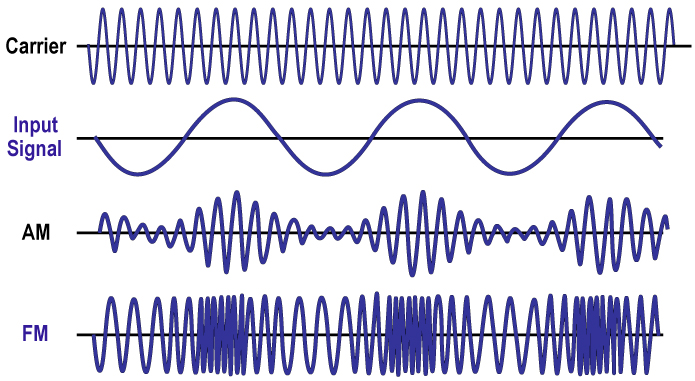
\includegraphics[width=\textwidth/2 + 3em]{images/modulation.jpg}
	\caption{AM and FM modulation of a Signal onto a Carrier {\protect\footnotemark}}
	\label{fig:mod}
\end{figure}
\footnotetext{Source: \href{http://www.hill2dot0.com/wiki/images/a/af/G0612_Carrier-Modulation-Te.jpg}{\texttt{http://www.hill2dot0.com}}}

\subsection{Antenna Gain and Impedance}
Antenna Gain is closely related to the antenna's directivity, means it corresponds to how concentrated the radiated power is in one specific direction. 
Gain, however, is the product of the antennas efficiency and the directivity, and is usually measured in direction of the highest
To maximise the radiated power by an antenna, it is important to "match" the impedance of the antenna to the electric circuit, since antennas are resonant devices, e.g. a part of the input power at the antenna will be reflected, which can introduce a whole range of problems, especially when high power is transmitted/reflected back to the transmitter. This reflected power can be minimised by so-called impedance matching, where the impedance of an antenna relates the voltage and current at the input of the antenna.\\

\subsection{VSWR}
\label{sec:vswr}
As stated in the last section, not all of the input power is radiated by the antenna, but is partially reflected. The mismatch of a load $Z_L$ to a source $Z_S$ can be expressed with the so-called \textit{reflection coefficient}:
\begin{equation}
	\centering
	R = \frac{Z_L - Z_S}{Z_L + Z_S} = \frac{V_{incident}}{V_{reflected}}
\end{equation}

Using this reflection coefficient, the \textit{Voltage Standing Wave Ratio} can be calculated. The VSWR is a common term to express how efficient the power is transmitted from the power source into the load. In physical terms, the VSWR measures the ratio between the highest and lowest voltage (basically the voltage variance) across the transmission line. If there is no reflected power, e.g. all of the power is transmitted, then no interference of the original signal and the reflected occurs. This results in a VSWR of 1. However, if there is some power reflected this will cause constructive and destructive interference with the input signal, which will result in a $VSWR \geq 1$. It is important to note that the VSWR is depending and varying with the frequency, since the impedance will change with increased or decreased frequency.
In practical terms, the VSWR can be calculated as
\begin{equation}
	\centering
	VSWR = \frac{1 + |R|}{1 - |R|}
\end{equation}
The Power Loss due to this reflection can then be calculated using the VSWR:
\begin{equation}
	\centering
	L_{return} = 20 \log_{10}{\frac{VSWR-1}{VSWR+1}}
\end{equation}
To express this loss in terms of percentage of the input power, one can use so-called \textit{conversion tables} (see appendix), which allows to match a specific VSWR value to the Losses in Percent, or one can calculate it using the reflection coefficient and the following formula:
\begin{equation}
	\centering
	P_{reflected} (\%) = 100 * R^2
\end{equation}

\subsection{Transmitted Power}
\label{subsec:power}
After having introduced the VSWR and thus the true emitted \& reflected power, we now want to characterise and take a brief look at the power received at the receiver. In general, the Power received is governed by the following equation
\begin{equation}
	\centering
	P_r (dB) = P_e - L_C + G_1 + G_2 - L_P
	\label{eq:path}
\end{equation}
with $P_e$ being the emitted power in dB, $L_C$ the losses of a cable, if there is one in-between the antenna and the power source and $G_1$ and $G_2$ the Gain of receiving respectively emitting antenna. $L_P$ is the Path Loss, means the power that is lost due to transmission of power in the air. The Path Loss is dependant on the distance of receiver and emitter, but also on the frequency of the used signal. It can be calculated as follows:
\begin{equation}
	\centering
	L_P = 22 + 20\log(d\times\lambda^{-1})
\end{equation}

%%%%%%%%%%%%%%%%% TASK 2 %%%


\section{Experiments}

\subsection{Radio antenna \& Spectrum Analyser}
To perform all the experiments, we were provided a DSA800 Series Spectrum Analyser manufactured by RIGOL Technologies with a frequency range from 9 kHz to 1.5 Ghz and a resolution of 1Hz. 
%After a short introduction to the general usage, we tested the main functions of the Spectrum Analyser.
To familiarise oneself with the Spectrum Analyser, we used a simple Dipole Antenna and connected it to the Input of the Spectrum Analyser (SA). Using the full span of the SA we observed different peaks at different frequencies, shown on the screen of the SA - where the X-axis denotes the signal power in dB and the Y-axis the frequency (range). In general, the lowest observable power was about -60dB, which we considered as being the background noise.\\
By selecting the frequency range with upper and lower limits such as we were within the radio frequency band (between 85 and 110 MHz), we were able to see again peaks at different frequencies. After choosing one of the higher peaks and setting its corresponding frequency as center frequency, we used the Demodulation-function of the SA to demodulate the signal, which we expected to be frequency-modulated since this is the common modulation for conventional radio signals. By connecting a set of speakers to the audio output of the SA, we were able to hear the demodulated FM signal in the audible frequency spectrum.

By modifying and testing different resolution times we were able to increase the quality and steadiness of the audible signal. We performed the described procedure with multiple detected peaks in the radio band to test the reception of different modulated signals.



%%%%%%%%%%%%%%%%% TASK 3 %%%
\subsection{VSWR measurement}
To characterise three different dipole antennas and their efficiency, we measured the Voltage Standing Wave Ratio (VSWR). The SA itself can not measure the VSWR, but by connecting a VSWR-bridge, which essentially feeds the reflected power back to one of the SA's input, this measurement is made possible.\\
By setting the SA to the \textit{VSWR-measurement}-mode, where the SA automatically detects the connected VSWR device and creating a signal with the SA's build-in Signal Generator, the general setup for this measurement was done. The VSWR-bridge then had to be calibrated by using the calibration function of the SA. The calibration essentially measures the internal impedances, so that after connecting an antenna the internal impedances will not show up in the measurement.\\



\begin{center}
\begin{tabular}{l | c | c | c }
	& \textbf{Antenna 1} & \textbf{Antenna 2} & \textbf{Antenna 3}\\
	\hline
	Frequency & 433 MHz & 840 MHz & 840 MHz\\ \hline
	Peak & 457.5 MHz & 847.5 MHz & 836.5 MHz\\ \hline
	3dB BW & 42.5 MHz & 90.0 MHz & 102.5 MHz\\ \hline
	Reflected Power & 2.5 \% & 2.21 \% & 6.43 \% \\ \hline
	Return Loss & 16.0 dB & 16.9 dB & 12.6 dB\\ \hline
	VSWR & 1.38 & 1.35 & 1.68\\ \hline
\end{tabular}
\captionof{table}{Antenna characteristics for three omnidirectional antennas}
\label{tab:VSWR}
\end{center}

Comparing the Reflected Power of the three respective antennas we can see that all antennas are below 10\%, the threshold for an antenna being seen as having a good performance in terms of transmitting power.

%%%%%%%%%%%%%%%%% 

\subsection{Antenna Gain}
Having measured the Reflected Power for the three provided antennas, we now want to calculate the Gain of the antennas. This is done using a calibrated broadband antenna which has a Gain of 2.9 dBi as a transmitting antenna. The setup here is similar to the setup of the VSWR measurement, but now we do not use the VSWR bridge. Instead, we connect the transmitting antenna directly to the SA TX output and the receiving antenna via a short cable to the SA RX input. Now we set the transmitting frequency to the calibrated antenna's peak frequency of 840MHz and the SA's emitting power to 0 dB. Placing the receiving antenna at a distance equal to the wavelength ($\lambda = d = 35.714cm$) and measure the received power at the uncalibrated receiving antenna, we can now calculate the Gain of the receiving antenna with \cref{eq:path} given in \cref{subsec:power}.

\begin{center}
	\begin{tabular}{l | c | c}
		& Antenna 2 & Antenna 3 \\ \hline
		received Power (dBm) & -24.0 &  -26.3\\ \hline
		calculated Gain (dBi) & -4.4 & -6.7 \\
	\end{tabular}
	\captionof{table}{received Power and Gain at receiver antenna}
	\label{tab:gain}
\end{center}
Since the used calibrated broadband antenna did not support frequencies as low as 433 MHz, only the gain of two of the three antennas could be characterised using this method.
As for the losses in the cable we used a value of 0.5dBm, a value that was provided by the instructions.

The calculated Gain and the received power fit our VSWR measurements very well. One can easily see that Antenna 3 has a lower Gain value, which corresponds to our previous observation that Antenna 3 has higher return losses, c.f. \cref{tab:VSWR}.

%%%%%%%%%%%%%%%%% 
\subsection{Received Power vs. Distance}
To show the dependency of received power strength and distance between emitter and receiver, we used a small wireless remote, as is usually used for garage door opener. Since this device operates at around 433 MHz, we hooked Antenna 1 onto the Spectrum Analyser. Starting with a distance of $d=\lambda=0.693m$ in-between the transmitter device and the receiving antenna, we increased the distance in steps of $20cm$ each, and measured the power received at the Spectrum Analyser.
The received power plotted vs. the distance can be seen in \cref{fig:omni}
\begin{figure}[h!]
	\centering
	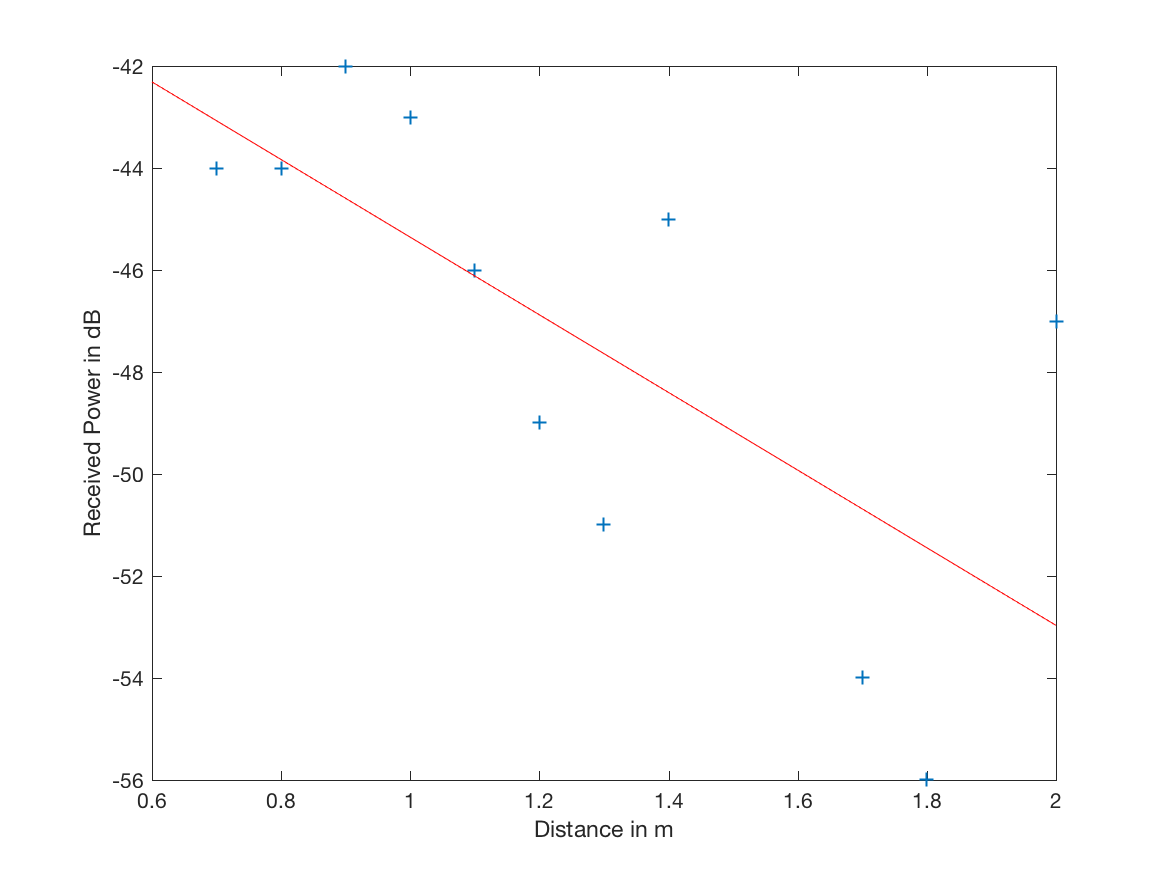
\includegraphics[width=\textwidth/2+5em]{images/omnidir.png}
	\caption{Received Power vs. Distance}
	\label{fig:omni}
\end{figure}
An observation we made, is that the received power fluctuates quite a lot. We expected the power to decrease more or less linearly, but the measured data looks very scattered. However, using a least-square linear approximation to the measured data, one can see a trend towards decreasing power with increased distance - which is what we expected.
The fluctuating power might be explained by having obstacles, e.g. multi-path effects, since the room we performed all the experiments, was not shielded. Also we noticed high variations in the measured power, depending where in the room we were standing - even when not standing in line-of-sight between transmitter and receiver.
Another reason might be, that the distance measurement was not as precise as we would have wished, since we used an ordinary table and a tape measure to measure the distance from receiving antenna to the transmitter.




\subsection{Antenna Gain Pattern}
The final experiment in this laboratory was the measurement of a high-precision high-gain antenna, the Hyperlog 7025 - in particular the radiation pattern in different directions covering a full 360° of the antenna was to be measured.
This was done by using the same setup as in the measurement of received power vs. distance, but this time the TX output of the SA was used to connect the Hyperlog antenna. Also, we exchanged the receiving antenna with the calibrated antenna, since the Hyperlog antenna is intended for using only frequencies within the range of 700MHz to 2.5 GHz.\\
Again, as emitting power we chose 0 dB and placed the emitting antenna at a distance of $d = \lambda = 35.7 cm$ from the receiving one.
The emitting antenna was also placed on a rotatable plate. The received power was then recorded at every 20°-step, until the full 360 degrees were covered. The result was then plotted and can be seen in \cref{fig:hyper}.

\begin{figure}[h!]
    \centering
    \begin{minipage}{0.45\textwidth}
        \centering
		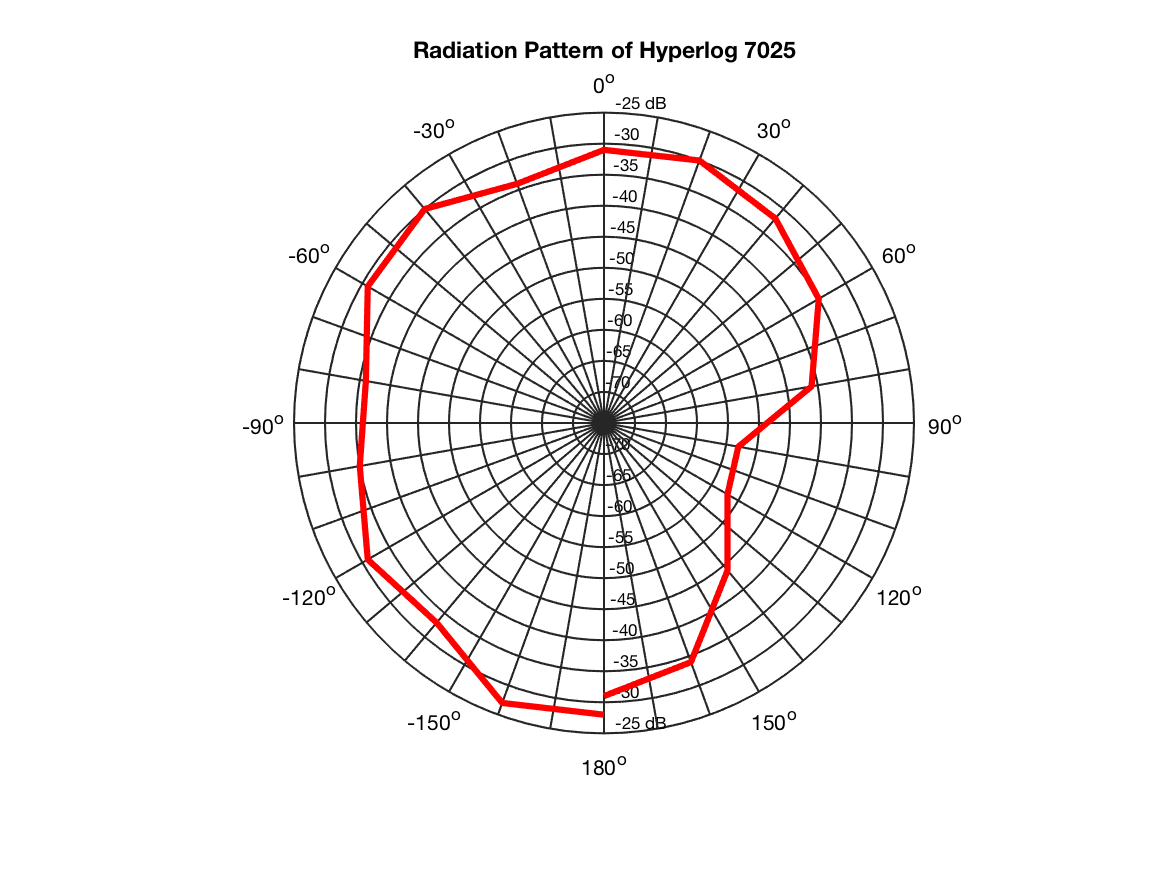
\includegraphics[width=\textwidth+6em]{images/hyperlog.png}
		\caption{Measured Radiation Pattern}
		\label{fig:hyper}
    \end{minipage}\hfill
    \begin{minipage}{0.45\textwidth}
		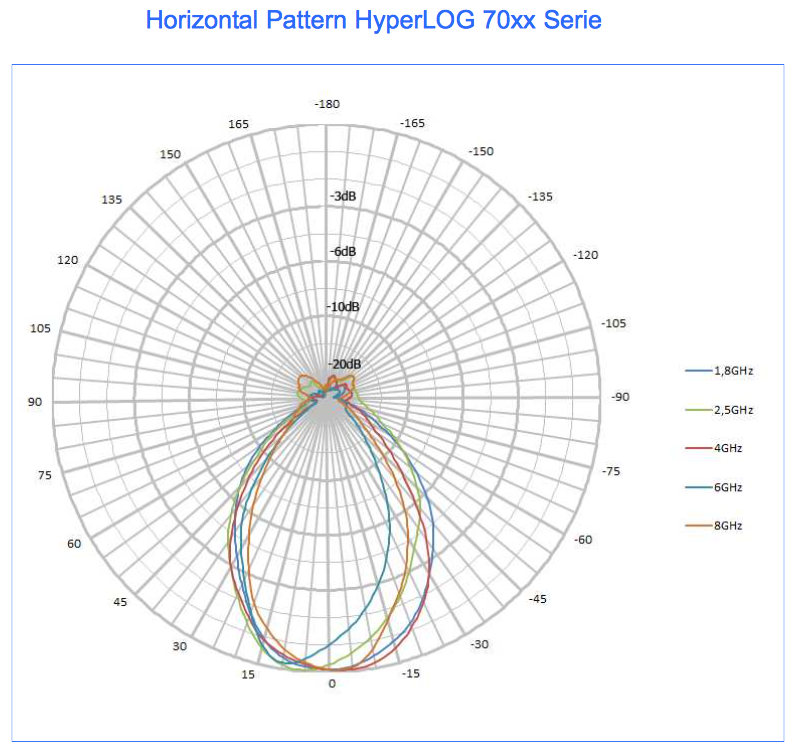
\includegraphics[width=\textwidth]{images/hyperlog_ds.png}
		\caption{Pattern according to data sheet\protect\footnotemark}
		\label{fig:hyper_sheet}
    \end{minipage}
\end{figure}

\footnotetext{\href{http://www.aaronia.com/Datasheets/Antennas/Directional_Antenna_Series_Aaronia_HyperLOG7000.pdf}{Source: device datasheet at \texttt{http://www.aaronia.com}}}

\Cref{fig:hyper} shows a quite shapeless blob that is more or less equally sized in every particular direction. This is very much the opposite of what we had expected, since a high-gain antenna is very directional. This expectation matches the official radiation pattern that is provided in the data sheet of the Hyperlog antenna (c.f. \cref{fig:hyper_sheet}). However, knowing the shape of the real we can see, that our measured data shows particular features of the real radiation pattern, especially a higher gain respectively a broader lobe in 0° direction\footnote{note: the measured data is plotted with a 180° shift compared to the plot from the data sheet!} - and a lower amplitude on the "sides" of the antenna (-90° and 90°).

These very strong deviations from the expected outcome can partially be explained by the quite poor measurement technique - in particular the turntable we used was not very stable and not best suited for the measurement since it did not provide any mechanisms to fix the antenna properly. This could have resulted in miss-pointing the antenna, leading to a poor signal reception of the receiving antenna -  we reasoned this issue as being the one most harmful for the measurement. Also, due to other emitting devices such as cell phones, computers, etc. the measurement could have been falsified. Multi-Path effect could also play a role in falsifying the measurement - especially during the pointing angles of about 180°, since the emitted Power could have been easily reflected towards the SA by the wall and other obstacles that were in the room.

However, a slight correlation between expected and real outcome can be seen, especially the slightly larger lobe towards the 0° pointing angle.


\section{Conclusion}